\section{Theorie}
\label{sec:Theorie}

Einige periodische Vorgänge in Raum und Zeit lassen sich durch
zusammengesetzte Sinus- und Cosinusfunktionen der Form

\begin{align}
  g(t) & = A\sin \frac{2\symup{\pi}}{T}t & h(t) & =
  A\cos \frac{2\symup{\pi}}{T}t \\
\end{align}
mit der Amplitude $A$ und der Periodendauer $T$ darstellen. Im Folgenden
wird das Fouriersche Theorem vorgestellt, mit welchem man solche Funktionen
zusammensetzen kann.

\subsection{Das Fouriersche Theorem}

Eine gleichmäßig konvergente Reihe der Form

\begin{equation}
  \frac{a_0}{2} + \sum_{n=1}^{\infty} \Bigl(a_n \cos
  \Bigl(n\frac{2\symup{\pi}}{T}t\Bigr)
  + b_n \sin \Bigl(n\frac{2\symup{\pi}}{T}t\Bigr)\Bigr)
\end{equation}
stellt eine periodische Funktion $f(t)$ dar.
Diese sogenannte Fourierreihe besitzt die Koeffizienten

\begin{align}
  a_n & = \frac{2}{T}
  \int_{0}^{T} f(t) \cos (n\frac{2\symup{\pi}}{T}t) \symup{d}t
  \\
  b_n & = \frac{2}{T}
  \int_{0}^{T} f(t) \sin (n\frac{2\symup{\pi}}{T}t) \symup{d}t,
  \label{eqn:anbn}
\end{align}
die jeweils für $n \to \infty$ gegen null gehen müssen, damit die Reihe
konvergiert. Diese Koeffizienten können auch gleich Null sein.
Für eine achsensymmetrische Funktion $f(t)$ beispielsweise sind alle $b_n$ null,
während für eine punktsymmetrische Funktion $f(t)$ alle $a_n$ null sind.
Werden die Amplituden der Fourierreihe in Abhängigkeit von der Frequenz
dargestellt,
so entsteht ein Linienspektrum wie in Abbildung \ref{fig:Linienspektrum}.

\newpage

\begin{figure}
  \centering
  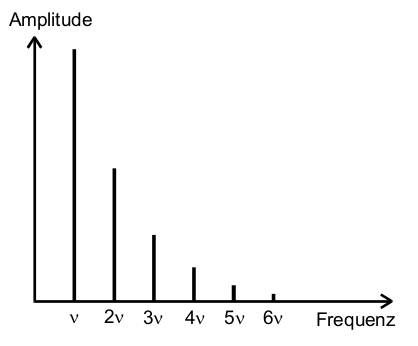
\includegraphics[height = 5cm]{Linienspektrum.png}
  \caption{Linienspektrum einer Fourierreihe mit der Grundfrequenz $\nu$\cite{anleitung}.}
  \label{fig:Linienspektrum}
\end{figure}


Bei dem folgenden Versuch wird die Fouriersumme bis zu einem endlichen
$n$ betrachtet. Dabei tritt eine endliche Abweichung zwischen der Stelle $t_0$
der Reihe und $f(t_0)$ auf. Diese Erscheinung wird als Gibbsches Phänomen
bezeichnet.

\subsection{Die Fouriertransformation}

Das Frequenzspektrum $g(\nu)$ einer periodischen Funktion $f(t)$ kann über
die Fouriertransformation

\begin{equation}
  g(\nu) = \int_{-\infty}^{\infty} f(t) \symup{e}^{\symup{i}\nu t} \symup{d}t
\end{equation}
berechnet werden.
Das Spektrum $g(\nu)$ hat die Gestalt einer konvergierenden Reihe von
$\delta$-Funktionen wie in Abbildung \ref{fig:Linienspektrum} dargestellt.
Mit der Umkehrung der Fouriertransformation

\begin{equation}
  f(t) = \frac{1}{2\symup{\pi}} \int_{-\infty}^{\infty} g(\nu) \symup{e}^{
  -\symup{i}\nu t} \symup{d} \nu
\end{equation}
kann aus dem Frequenzspektrum $g(\nu)$ die zugehörige Funktion $f(t)$ bestimmt
werden. Dies nennt man auch Fourieranalyse.
In der Praxis treten hierbei Abweichungen auf, da nur über einen endlichen
Zeitraum integriert werden kann.
